\cleardoublepage
\chapter{Floatable Blocks}\label{ch:floats}

% Required implementation:
% \begin{itemize}
%     \item extension of chapter 2 code to support floats
%     \item tradeoffs between Plass\cite{Plass1981} pagination and `dumb' pagination. Should floats be
%     `floatable'?
%     \begin{itemize}
%         \item how floatable?
%         \item how much effort do we put in before it stops being worth it?
%     \end{itemize}
%     \item Floats across multiple columns?
%     \begin{itemize}
%         \item simple multiples of galley width/line height
%     \end{itemize}
%     \item Bringhurst's suggestion\cite{Bringhurst2008} of making blocks take up multiples of the
%     leading to always keep text in phase (could even factor this into chapter 2 implementation)
% 
% \end{itemize}

The system described in Chapter~\ref{ch:malleable} supports only simple documents that are composed solely from text. Many (perhaps most) real-world documents contain figures, diagrams, illustrations, tables etc., and so consideration must be given towards how these should be handled.
This chapter extends the work of the previous chapter to allow floatable graphical blocks, whose absolute position within a document's text may vary, depending upon the layout.

\section{Implementation}

The implementation of the system described in the previous chapter is deeply rooted within \gls{pdf}, and requires a custom-written plugin (see Section~\ref{sec:acroplugin}) for Adobe Acrobat to view the documents. Consequently, it is difficult to test that particular implementation on any device which is not running Microsoft Windows and does not have a fully licensed version of Adobe Acrobat. Effectively, this rules out any mobile \ebook{} readers.

Almost all \ebook{} readers support the \epub{} format,\marginpar{Amazon's Kindle is one of the few devices that does \emph{not} support \epub{}} which is principally built upon \html{}, \css{}, and JavaScript. With this in mind, it was decided to reimplement the system using these technologies, in order that it could be tested on \ebook{} hardware. 



\subsection{Document Generation}
\label{sec:docgen}




In the system described in the previous chapter, the generation of malleable documents had been a rather labour-intensive process, involving the processing of the source document through \troff{} and \pdfdit{}. In the case of documents with galleys of more than one width, modifications needed to be made, by hand, to the document structure tree of the resultant \gls{pdf} files.

Adding or removing characters to the source of a \gls{pdf} file is no trivial matter, since the \textsc{xref} table, which stores the byte offsets of all \glspl{COSObject} within the file, is no longer correct. (Acrobat does kindly offer to fix this problem if it detects it, but it has the side effect of discarding any data it does not recognise. Clearly losing the document structure tree is undesirable.) The \textsc{xref} table can either be fixed programatically, or by a painstaking process involving a hex editor and a lot of patience. Significant lack of patience meant that there was only ever one multiple galley-width test document produced for the previous system.

Since the new system no longer relies on \gls{cog}-\gls{pdf}, the reliance on \troff{} and \pdfdit{} is no longer present. Consequently, a sensible approach is to produce a completely bespoke typesetting tool, allowing unneeded features to be removed, and the provision of some finer-grained control over other aspects. For example, it is important for this system that the the line-breaking and hyphenation algorithms can easily be changed.



In the new system, the source document is described in terms of separate logical blocks; a block is either designated as a `float', or as a `paragraph'. (Listing~\ref{lst:sourcedoc} contains an excerpt from a sample source document.) Floats are currently limited to referencing images only (with an optional size parameter). Paragraphs, on the other hand, are described by their desired textual content. This is deliberately simplistic. It is envisaged that in a real system, the source document would have a richer language, perhaps marked up in a form similar to \LaTeX{} source, or in \xml{}.

\begin{lstlisting}[label=lst:sourcedoc,captionpos=b,float,caption={[An excerpt from a sample source document]An excerpt from a sample source document, itself an excerpt from \cite{Pinkney2011}. The document is parsed from top to bottom. Paragraphs are separated by blank lines. Floats are specified by lines that begin \texttt{\_\_FLOAT} and contain a reference to an image. Subsequent lines, until the next \texttt{\_\_FLOAT} or \texttt{\_\_PARA} marker, are assumed to be the float caption.}]
3.1.3 pdfdit

Having generated the source document, it was processed with
ditroff to generate the intermediate code used to feed each
typesetter post-processor. This output is very expressive, and,
unlike TEX's DVI, contains enough information that post-
processors are easily able to locate the start and end of lines
and paragraphs within the document. This meant that only minimal
changes were needed to be made to the pdfdit package described in
[1] to implement our design.

__FLOAT fig4.png

Figure 4: Sample renderings from the Acrobat plugin at page
widths of 42, 48, and 54 em.

__PARA

The first change necessary was to decrease the granularity of the
output COGs, producing them at the line level, rather than at the
paragraph level. Secondly, some method of generating the
requisite tree representing the document structure was required.
This was solved by simply using the point at which the original
version of pdfdit would have started a new paragraph-level COG,
and, instead, starting a new paragraph-level block entry in the
document structure tree. Each subsequent line-level COG produced
can then be added as a child of this block.

Once the entire output file has been parsed, the tree
representations of the various width galleys are amalgamated
per-paragraph, as indicated in figure 3, and finally the PDF file
is serialised, replete with COGs and content tree.

\end{lstlisting}


 Next, the source document is passed through a program\marginpar{Should I find a name for this program? It's a bit unwieldy referring to it anonymously all the time. Is \emph{Galley Renderer} ok? Or \emph{Document Generator}?} to produce the output that becomes the malleable document itself. This program passes the text of each paragraph through an implementation of a line-breaking algorithm (we use Knuth-Plass, but this could be replaced by any other algorithm that performs line breaking and justification). Each paragraph is rendered multiple times, once for each galley width, in order to produce the document's multiple galley renderings. Each line of each rendering of every paragraph is converted into a list of its composite words. All of these words have an associated offset value, which is later used when drawing the text to ensure that each word is positioned on the line with the correct spacing. The general algorithm used is given in listing~\ref{lst:parsplitter}.


\begin{lstlisting}[label=lst:parsplitter,captionpos=b,float,caption={Algorithm followed by the galley renderer}]
 TODO: write theI haven't written this yet :(
\end{lstlisting}


The content of the floats is largely left unchanged. A reference to the image, along with its required dimensions, is simply passed through to the output. If dimensions were not explicitly specified in the source document, the pixel size of the image itself is used.

Finally, once the whole of the source document has been processed, the rendered content is output\ed in the form of the document structure tree shown in figure~\ref{fig:tree}\ed encoded in JSON. This becomes the data representing the source document, which, in conjunction with the viewer defined in the next section, becomes a \emph{malleable document}.




\subsection{The Viewer}
\label{sec:viewer}

In order to circumvent the browser's default text layout algorithm, and to ensure that our ``high quality'' pre-computed text-layout is used, the viewer must specify the absolute position of every word on each line, in a manner not dissimilar to the internals of a PDF file. The document generator described in the previous section ensures that all the information needed to lay the text out is contained within the generated JSON data representing the document structure tree.


When the viewer is launched, it decides which is the most appropriate galley rendering to display, based on a metric of which rendering will be most aesthetically pleasing. Since it appears to work well, the metric defined in Chapter~\ref{ch:malleable} is used, which attempts to balance a penalty for excessive inter-column whitespace against a penalty for too many columns. 

Although every galley is rendered in the same point size, this can be scaled up or down at view-time, based on the preference of the user, to simulate point-size changes. The gaps between words are scaled proportionally, to allow the text to remain correctly justified.




\subsubsection{Floats with a Queue}
The first attempt at supporting floats took inspiration from \TeX, which places floats into a queue until it finds somewhere it deems appropriate to place the first float. In order to emulate this, two queues were defined: the \emph{float queue}, and the \emph{line queue}. (`Line queue' is perhaps a slight misnomer, but it is somewhat snappier than `non-floating items queue'.)


If both queues are empty, as they will be at the start of the layout process, the document structure tree is traversed, and when the first paragraph-level item (see figure~\ref{fig:tree}) is encountered, its subcomponents (of the chosen galley rendering) are added to the requisite queue: lines to the line queue, and floats to the float queue.

When at least one of the queues is not empty, document layout begins. If the float queue is non-empty, and the first float in the queue will fit below the last typeset item, it is placed on the page. If not, items from the line queue are placed one by one, until no more will fit in the current column. When this happens, a new column is started, and the first float in the float queue is output. Whenever the line queue is depleted, and no floats in the float queue will fit at the current point on the page, all subcomponents of the next paragraph-level item from the document structure tree are queued. This process is illustrated in Figure~\ref{fig:float-flowchart}.

\begin{figure}
  \begin{center}
  \includegraphics[height=\textheight]{gfx/floatqueueflowchart}
  \end{center}
  \caption{Flowchart describing the two-queue float algorithm}
  \label{fig:float-flowchart}
\end{figure}

Pagination is reasonably simple with this queueing system: as soon as a page is full, the layout can be restarted at the origin of the page using the current status of both queues and the document structure tree. It is entirely possible that floats may appear on pages subsequent to their callout point in the text, but this effect should be no worse than in many current typesetting systems.

While this approach does produce reasonable layouts, and handles floats well without the need for backtracking, it is not particularly conducive to producing layouts with floats that span multiple columns. The queue-based layout described above is rather simplistic: it knows about the size of each component that it lays out, but it does not remember the history of the positions of any of the components that are already laid out. This makes it difficult to have items that span more than one column, because there is no mechanism to mark space on the page as being reserved. In order to do this, another approach must be taken.

\subsubsection{A Grid-Based Layout}
% - Support of floats
    % - Queue system
    % - Grid/array system (no need for queue)
    % - Multicolumn floats
        % - issues with spanning \& pagination
A simple method for allowing parts of a page to be reserved is to break it up into a grid. Grid-based layouts are useful in many situations~\cite{Collier1991}; one example of particular note is that of modern-day newspapers (see figure~\ref{fig:gridlayout}). Following the example set by these newspapers, the grid used in this system is defined to have a row height of the leading of the document's body text, and a column width of the measure of one text column plus the required gutter space.

\begin{figure}
    \includegraphics[width=\textwidth]{gfx/newspaper}
    \caption[An example of a grid-based layout]{An example of a grid-based layout in a UK newspaper. Note how all the baselines of the main body text are aligned to a common grid, and that all items span integer multiples of columns.}
    \label{fig:gridlayout}
\end{figure}

The viewer uses the dimensions of the float, as specified in the document structure tree (see section \ref{sec:docgen}), to determine how many columns it should span. The float is scaled to span the integer multiple of column widths that most closely matches its `natural' size, though for reasons that should hopefully be obvious, this number is limited to a minimum of 1, and a maximum of the number of columns on the page. Additionally, checks are made to ensure that the scaling will not cause the height of the figure to exceed that of the page.

An advantage of this grid-based approach is that it no longer requires the use of queues, either for lines, or for floats. The viewer simply traverses the document structure tree, placing each item in the first available place in the grid. In the case of floats, or other items larger than multiples of the main leading, spaces in the grid can be marked as reserved, to prevent other items from trampling over their reserved space. If a float will not fit directly below the previous item to be placed, the grid is walked over until a gap of sufficient size can be found. Figure~\ref{fig:screengrab} shows an example of a document laid out with this system.



\begin{figure}
    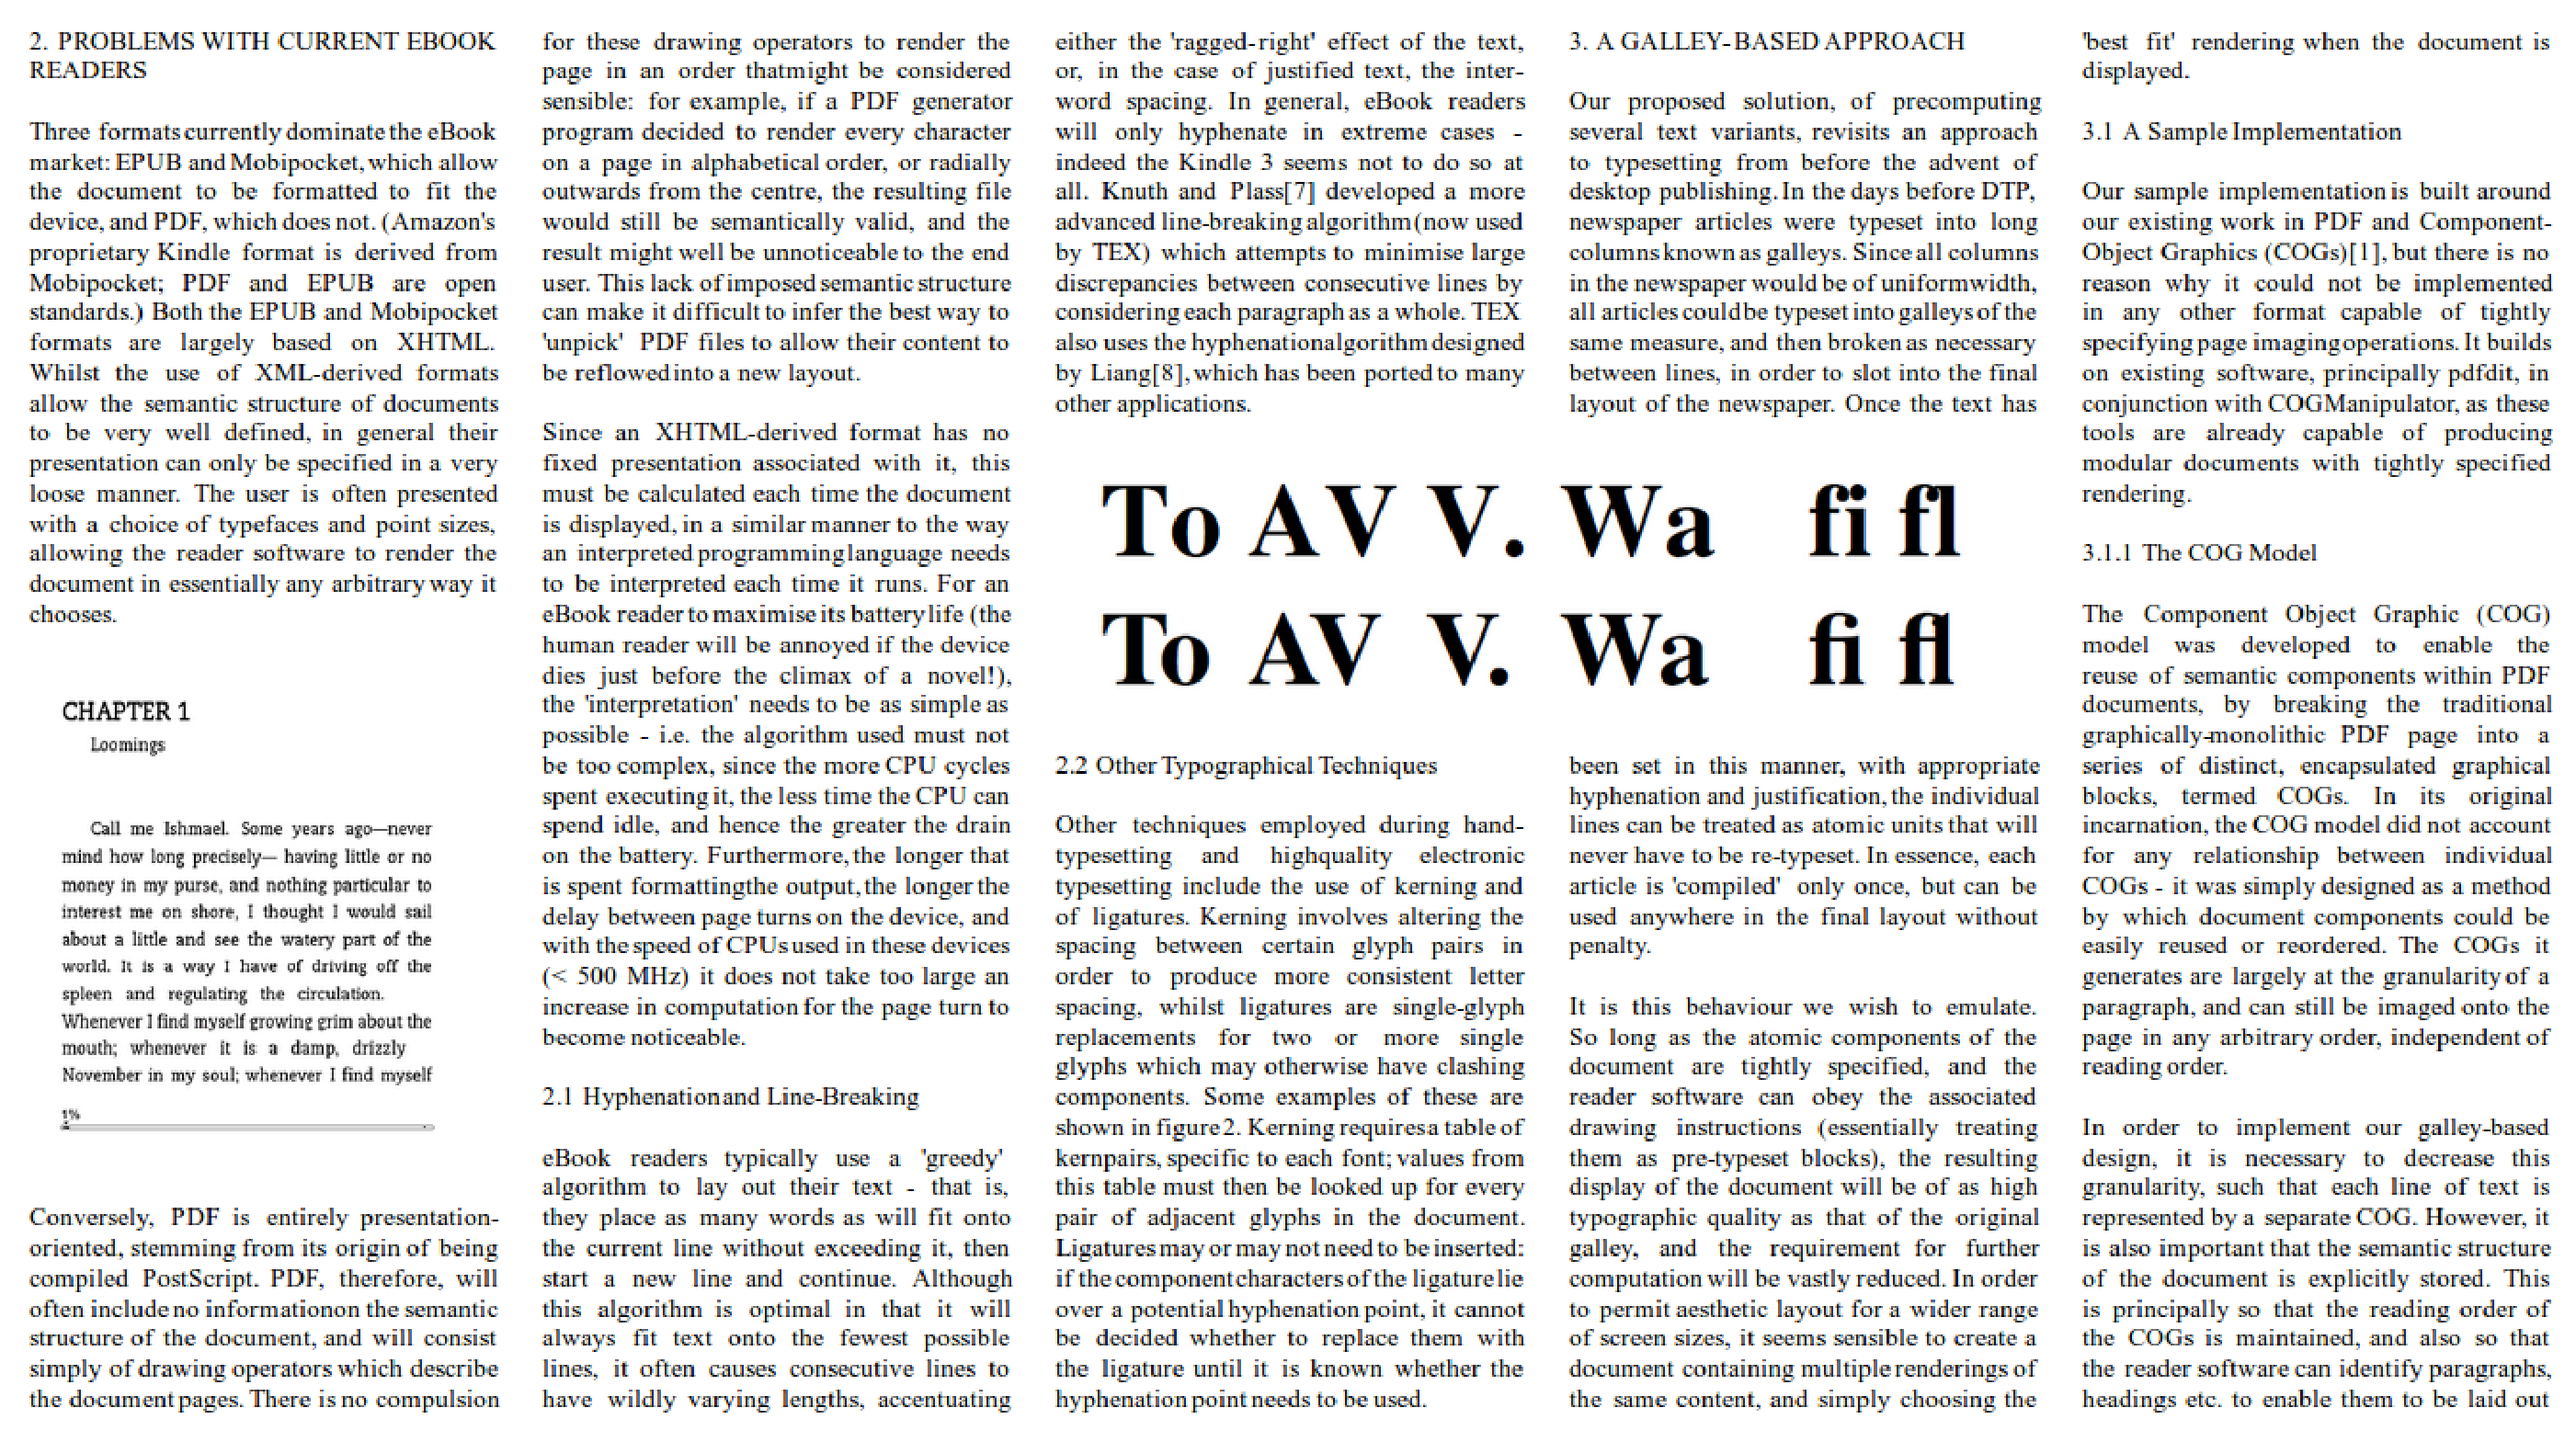
\includegraphics[angle=90,origin=c,width=\textwidth]{gfx/floatrendering}
    \caption[A sample rendering with multi-column floats]{An excerpt from \cite{Pinkney2011}, typeset and rendered by our new system.}
    \label{fig:screengrab}
\end{figure}

Pagination becomes a little trickier when floats are allowed to span multiple columns. For example, if a float, whose natural size would lead it to span $n$ columns, is encountered in the document structure tree when there are $(n-1)$ or fewer columns remaining to be typeset on the page, it must be decided how best to handle the situation. Three obvious options present themselves: alter the float to span fewer columns; delay the placement of the float until the start of the next page; or backtrack and check whether there is room to move the float back one or more columns, by shunting non-floatable text lines forwards.

The first option is clearly not desirable behaviour, given that shrinking a float may well reduce its legibility. Additionally, if this becomes a common problem, it it likely to be noticeable that floats spanning into the rightmost column of the page appear shrunken. The second option (delaying placement until the following page) is a reasonable compromise, though it will increase float-drift (whereby floats become separated from their callout points in the text), which is not ideal. The third option (backtracking and shunting) is likely to produce the most desirable output, although some computational overhead will be added. One approach is simply to check whether there is enough space immediately to the left (specifically a gap between other, already placed, floats) into which the current float can be placed, with the displaced lines being shunted forwards. This method will not produce layouts as optimal as methods that use full backtracking and check all possibilities, but it will run in much quicker time. A combination of all three of the above options is likely to work best in practice.


